\subsection{UDP Losses}
Previously, we have seen that while, the udp sender is sending 100Gb/s of BW the receiver is seeing effectively 0 bytes in userspace. This phenomena was always observed, regardless of whether the netserver cpu was shared with the NAPI/irq cpu or not.

State I:  vanila 4.17: 
device driver reports 98Gb/s packets sent.
/proc/net/dev* reports high numbers of rx-drop packets.
netserver reports tens of Mb/s received. 

state I fix: Apparently  there is  a NET\_FLOW\_LIMIT**, which was dropping our packets.
There is a bit mask that controls whether the flow limit is active or not, but the only thing that helped was compiling the kernel w/o this option.

Result: The counter for rx-dropp was no longer rising. 

State II: vanila 4.17 w/o net\_flow\_limit.
device driver reports 98Gb/s packets sent.
netserver reports tens of Mb/s received.
dropwatch*** reports ip\_defrag as the main "hub" for dropped packets.

state II fix: There were several changes introduced between 4.16 and 4.17. Eric Dumazet, from Google was working DDOS prevention, where ip\_defrag was the target.
The fix was; increasing the number of buckets:
sudo sh -c "echo 16000000000 >/proc/sys/net/ipv4/ipfrag\_high\_thresh"
Result: 
Driver started reporting on ~50Gb/s received packets while netserver was seeing about 25Gb/s. Due to packets lost in transit, ip\_defrag was now dropping packets that couldn't be reassembled. And yes, pause parameters are configured both on the sender and the receiver. The driver was now slower than the network and packets would get lost. 

fix II: I've modified the test to send 8KB udp packets, more system calls but no need to defrag the packets.

Result: Driver started reporting 42Gb/s received, with netserver reporting 38Gb/s.
dropwatch was now pointing to udp\_enqueue. Increasing the receive socket size
brought the netserver report up to 42Gb/s.
The short version of the above is that three things needed to maintain sane UDP RX results. The first thing that must be fixed is the NET\_FLOW\_LIMIT issue, the second thing is the size of received packets and the third is the size of the UDP socket.
The open question is; weather, its possible in software to decrease the number of lost fragments in flight. With PFC on this shouldn't have been an issue.

\subsection{More Questions}
Possible things that maybe beneficial to look at, table \ref{tab:open_issues}.
\begin{table*}
\centering
\begin{tabular}{l|l}
Issue & difficulty/impact \\\hline
Huge pages in \oursys & Few days of work expected <+5\% improved performance \\
Inline functions & a known issue in the Linux community, a small study maybe in order\\
PFC & PFC has an impact on TCP performance, never looked at why\\
ad hoc driver memory reuse & motivation?\\
ad hoc NAPI budget & minor but could be interesting\\
UDP fragment losses & Not sure there is a resolution in SW\\
lock in TX queue & if were dealing with locks alreaady...\\
coalescing & with higher rates may be its time to reveisit?\\
New Theory: Add triger to NAPI call with TX Ring watermarks? & Awsome for TX and should also work for TCP\\
Is send more used? & batching in send, could show up to +5\%\\
TCP flows & why more than one flow needed to saturate single core?\\
Is prefetch usefull&\\\hline
\hline
\end{tabular}
\caption{\label{tab:open_issues}Open issues}
\end{table*}

\begin{figure*}
    \centering
    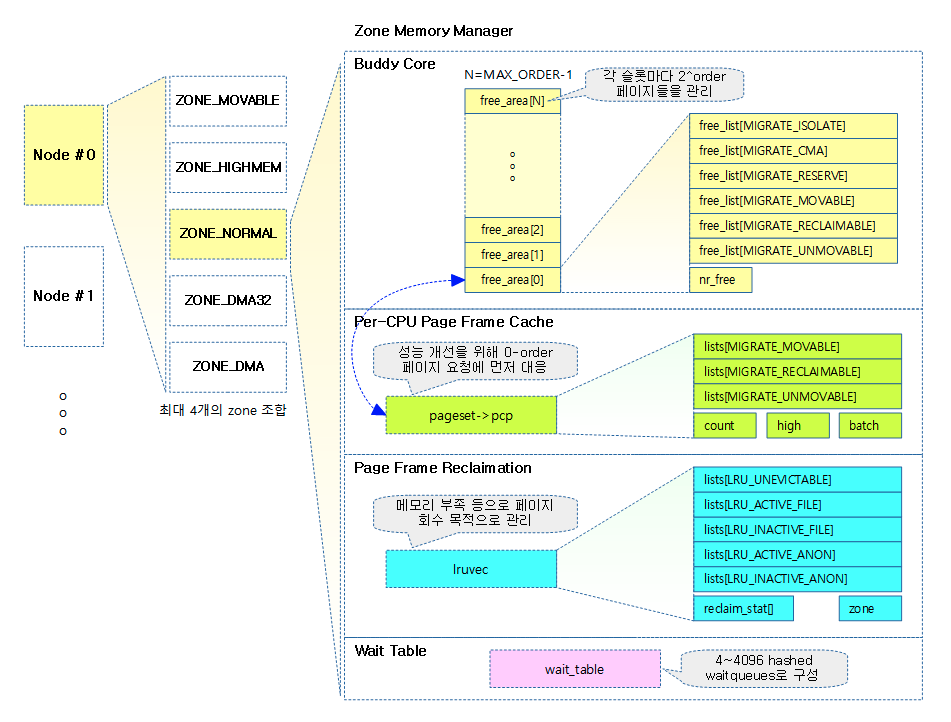
\includegraphics[width=1\textwidth]{figures/zoned_memory.png}
    \caption{Zoned memory allocator}
    \label{fig:zoned_memory_alloc}
\end{figure*}